\section{Raw Waveform Based Encoding}

A subset of deep learning research has focused on waveform-based methods and encoding music audio directly as raw time-series audio data.

\vspace{0.5cm}
\framebox[1.1\width]{
    \begin{minipage}{0.8\textwidth}
        Deep Neural Networks (DNNs) are a type of neural network with multiple hidden layers between the input and output layers. They are well suited for learning complex functions humans or other artificial neural networks cannot intuitively see from large datasets.
    \end{minipage}
}
\vspace{0.5cm}

There are many potential benefits to crunching low-level audio data. Firstly, information discarded from spectrograms (a representation discussed later in \ref{sec:fourier_methods_and_spectrograms}), e.g. phase, is not lost. Secondly, using raw audio does not limit the number and depth of features that can be learned, meaning such a model could potentially learn the intricate features of the human voice.

One of the problems of waveform based models is their lack of long term structure; this is caused by the sampling period being so short and the many thousands of samples that make up one continuous raw audio track\cite{JukeboxWebsite}.

\subsection{Jukebox}
\label{sec:jukebox}

The most influential model employing waveforms for music sound synthesis is called Jukebox\cite{Jukebox}. The Jukebox model is a deep neural network that learns to reconstruct music's vocal (and instrumental features) features from the raw audio data.

What is significant about the paper is its method of attempting to overcome the lack of long term structure. An autoencoder compresses input raw audio at the Nyquist Frequency to a discrete space using a technique called Vector-Quantized Variational Autoencoders (VQ-VAE)\cite{Jukebox}.

\vspace{0.5cm}
\framebox[1.1\width]{
    \begin{minipage}{0.8\textwidth}
        The Nyquist frequency is the highest frequency that can be represented by a sampling rate of an encoded audio signal so that the original signal can be reconstructed\cite{ProbabilityAndStatistics}.
    \end{minipage}
}
\vspace{0.5cm}

Several independent VQ-VAE levels are used, retaining different levels of resolution up to 128x encoding. Lower levels capture local music structures, e.g. timbre and local pitch, whereas higher levels capture higher-level long-range music structure features.

Each level is then trained using a sparse transformer-based model to learn the probability distribution of the VQ-VAE at each level of resolution. Finally, each VQ-VAE code is conditioned using the higher-level code during upsampling. Doing this enables the reconstruction to use all the VQ-VAE levels.

The model can be conditioned on lyrics, genre, and artist during inference. Inferred music features singing, instrumentals and some resemblance to a long-term structure. Music vocals (and language) are also synthesised and sung by the model on its own accord.

\begin{figure}[H]
    \centering
    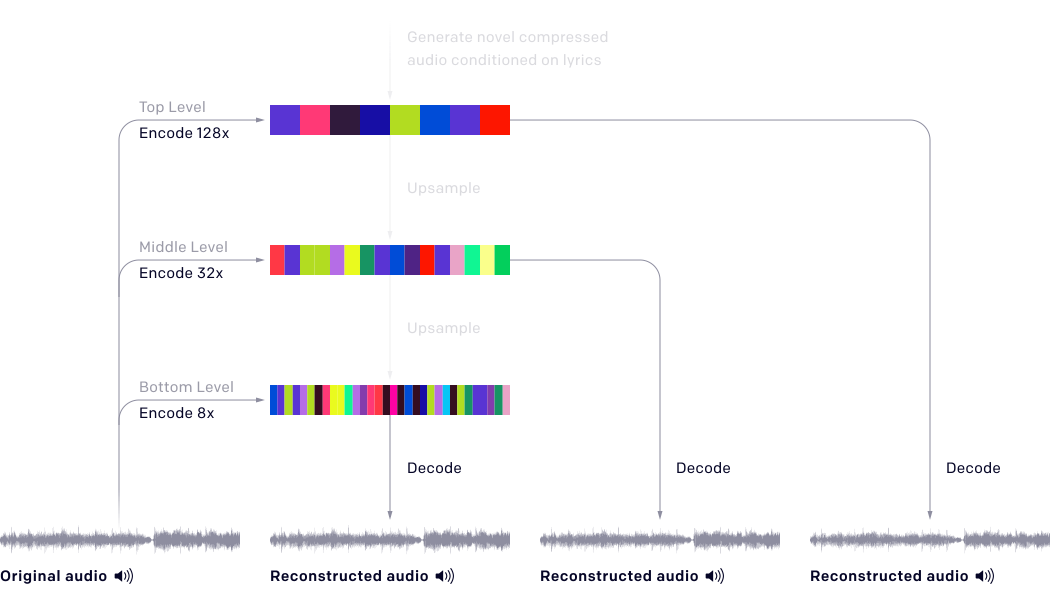
\includegraphics[width=0.8\textwidth]{literature_review/vq-vae.png}
    \caption{VQ-VAE Encoding and Compression: Successive levels further compress the raw audio data, discarding irrelevant information\cite{Jukebox}}
    \label{fig:jukebox_example}
\end{figure}

\subsection{Critical Evaluation}

Although local musical coherence and timbre are good in Jukebox, the longer-term musical structure is not fully present. The upsampling process also introduces significant noise into the final audio, which sounds jarring to the listener. Another significant disadvantage is the sheer size of the model, caused by the high volume of low-level time-series data). This large size means it takes multiple hours to infer one minute of music. This slowness limits its broad applicability as it is prohibitively expensive and prevents real-time applications, two significant issues to commerciality.

The model also functions much like a black box, preventing us from gaining any critical information about how it is synthesising its audio. This further limits its potential uses as we cannot independently modify model parameters such as the pitch and timbre of generated music. Finally, waveform based models require significant training data to train the model and extract relevant musical features accurately.

Sadly the lack of real-time features and prohibitively large model size limit Jubebox's potential applications. Any real-world application needs to be real-time or near-realtime.